\documentclass[11pt]{article}
\usepackage{hyperref}
\usepackage{pgfplots}
\usepackage[margin=0.5in]{geometry}
\begin{document}

\title{Hackintosh on a Dell T7500}
\author{Dr Ahmed Riza}
\date{}
\maketitle

\section{Requirements}
The machine I have is a Dell T7500 with an Nvidia Quadro 4000 GPU.  The extra items I have added to the machine since was a second Nvidia graphics card (an old GeForce 7900GS) and a SAS 6Gb/s PCI card.

{\bf Firstly, I had to remove the GeForce 7900GS, since OS X would not boot with the two cards present}.

\section{Preparation}
\label{prep}
I followed the excellent article at the following URL:
\url{http://lifehacker.com/5841604/the-always-up+to+date-guide-to-building-a-hackintosh}.  I followed this guide, until the end of Step 2.

\section{Specific Hardware}
The specific hardware on the T7500 that did not work out of the box are given below, and I'm going to address how I got them working in this article.
\begin{enumerate}
\item Nvidia Quadro 4000
\item Broadcom 5754 On-board Ethernet 
\item Enabling TRIM on the SSD drive
\end{enumerate}
Note that I do not have sound working yet, and I'll update this article once I get that working.

\section{Install OS X}
After booting from the USB stick prepared as described in the article referenced in Section~\ref{prep}, I installed OS X on a new Intel SSD 480 GB drive.  The installation went fine without any issues apart from my on-board Ethernet card not being recognized.  I just asked the installer to ignore Ethernet and the rest went smoothly.

However, after rebooting, I ran into trouble straight away.  There are a lot of forum posts from users who have had this experience, i.e. the machine starts booting with the Apple logo up and a spinning wheel.  After a while, all you will get is a black screen!

I researched all the forums I possibly could, and thought long and hard about what could be causing this, since this card is definitely supposed to work, and there are people who have it working on their machines.   So let's fix this.

\section{Nvidia Quadro 4000}

Confusingly, there are two varieties of this card, i.e.
\begin{enumerate}
\item Nvidia Quadro 4000
\item Nvidia Quadro 4000 for Mac
\end{enumerate}
I have the first kind, i.e. a non-Mac version.  I actually do not know the difference between the two cards. I believe it has something to do with the on-board ROM in the two boards.  There are people on the net who falsely claim that the non-Mac version would not work with OS X.  This is clearly wrong.

Anyway, the single source of information that finally lit the lightbulb in my head is the following, and I have to thank the author immensely for spending time to explain as he did.
\url{http://olarila.com/forum/viewtopic.php?f=18&t=154}. Here are the steps I took to get the GPU working.
\begin{enumerate}
\item Boot into OS X from the USB stick in safe mode.  That is, pass the ``-x'' parameter as a boot flag on the boot screen.

\item Install the Quadro 4000 driver from the Nvidia website.  Note that you will have to select the Quadro 4000 Mac card in order to download the driver. This is fine, since the driver will work with the non-Mac card, after a bit of modification as described below.   When the installation finishes, the installer will prompt you to reboot the machine.  Do not reboot yet, until we fix the driver.

On a side note, you may be wondering how I was able to install the driver from the Nvidia website, given that I do not have Ethernet working on this machine.  I simply downloaded it from another machine, and transferred via a USB stick.

I already knew the Vendor/Device ID of this card, by inspecting the hardware details from Windows.  In any case, the details are as follows:
\begin{itemize}
\item Vendor ID = 0x10de
\item Device ID = 0x06dd
\end{itemize}
We need to modify the Info.plist of the graphics driver with these values.  So, open up the Info.plist of the driver using your favorite editor.  Please note that the file is owned by root, so you'll need to {\em sudo} to modify the file.  I assume you know all about that.  I used vi to edit the file:
\begin{verbatim}
sudo vi /System/Library/Extensions/NVDAGF100Hal.kext/Contents/Info.plist 
\end{verbatim}
Look for the key {\bf IOPCIMatch}, and modify the string as follows:
\begin{verbatim}
<key>IOPCIMatch</key>
<string>0x000010de&amp;0x000006dd</string>
\end{verbatim}
Save the file and ``touch'' the Extensions folder:
\begin{verbatim}
sudo touch /System/Library/Extensions
\end{verbatim}

\item Now, we need to figure out the right value to pass to the {\bf PCIRootUID} boot flag.  Open a terminal and type the following command:
\begin{verbatim}
ioreg -l | grep -15 "AppleACPIPCI\ " | grep UID
\end{verbatim}
On my machine, I got two values, i.e. 
\begin{verbatim}
UID = 4
UID = 38
\end{verbatim}
After a bit of trial and error, what worked for me was the first value, i.e. {\em PCIRootUID = 4}.  \end{enumerate}
We are now ready to reboot, so reboot the machine.   I am still booting from the USB stick, so pass the following boot flags:
\begin{verbatim}
PCIRootUID=4
\end{verbatim}
The actual value you pass here depends on what was discovered in the step above.
That should get the Quadro 4000 working and finally, have a working machine with a nice GPU!

\vspace{1cm}
%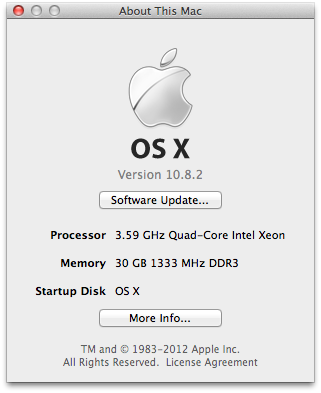
\includegraphics[scale=0.5]{screen-1.png}

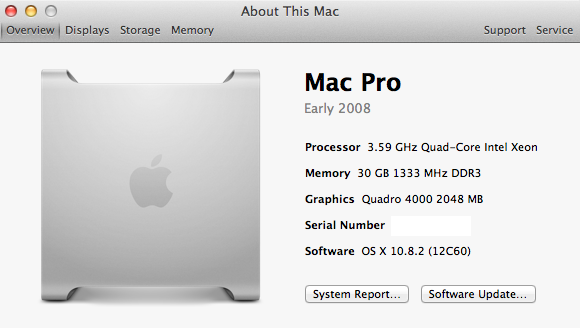
\includegraphics[scale=0.65]{screen-2.png}

\section{Broadcom 5754 On-board Ethernet}
This was the next challenge.  Some Googling revealed that a very nice person has actually written a driver for OS X.  
\begin{enumerate}
\item You can either download the precompiled driver from the following site:
\url{http://www.insanelymac.com/forum/topic/247470-bcm5722-bcm5754m-bcm5755m-bcm5787m-and-bcm5906m-nic-driver-3264-bit/}

\item Or compile it yourself with Xcode by downloading the source from git:
\url{https://github.com/adlan/BCM5722D/}
\end{enumerate}
Now, the driver may work straight out of the box for you, but chances are that it won't as was the case with me.  So, I booted into Windows, and found out the Device ID of the Ethernet card.  My card details were:
\begin{enumerate}
\item Vendor ID: 14e4
\item Device ID: 1681
\end{enumerate}
It is the Device ID, you'll have to enter into the Info.plist of the driver.  I was also a bit confused about where to install the driver.  I could not find this mentioned in the driver documentation or source code.   Some Googling revealed that it has to be installed under the
{\bf /System/Library/Extensions/IONetworkingFamily.kext/Contents/PlugIns/} directory.

So, I edited the Info.plist as follows:
\begin{verbatim}
sudo vi /System/Library/Extensions/IONetworkingFamily.kext/Contents/PlugIns/BCM5722D.kext/Contents/Info.plist
\end{verbatim}
I added an extra line to the dictionary containing the Device IDs:
\begin{verbatim}
                        <array>
                                <string>pci14e4,165a</string>
                                <string>pci14e4,167a</string>
                                <string>pci14e4,1672</string>
                                <string>pci14e4,167b</string>
                                <string>pci14e4,1673</string>
                                <string>pci14e4,1681</string>
                                <string>pci14e4,169b</string>
                                <string>pci14e4,1693</string>
                                <string>pci14e4,1712</string>
                                <string>pci14e4,1713</string>
                        </array>
\end{verbatim}
The entry with {\bf pci14e4,1681} is what I added.  After this, ``touch'' the Extensions directory as usual, reboot and Ethernet worked flawlessly.  Once again, many thanks to the author of the driver.

\section{Enabling TRIM on the SSD Drive}

This was the easiest job of all.  Once again, a very nice person has detailed the steps precisely and all I did was follow those steps to the letter.  The following page helped in that regard: \url{http://digitaldj.net/2011/07/21/trim-enabler-for-lion}.  I will detail the steps from this article, here for reference:

\begin{enumerate}
\item Backup the files wet are patching.
{\scriptsize
\begin{verbatim}
sudo cp /System/Library/Extensions/IOAHCIFamily.kext/Contents/PlugIns/IOAHCIBlockStorage.kext/
Contents/MacOS/IOAHCIBlockStorage /System/Library/Extensions/IOAHCIFamily.kext/Contents/PlugIns/
IOAHCIBlockStorage.kext/Contents/MacOS/IOAHCIBlockStorage.original
\end{verbatim}
}

\item Patch the file to enable TRIM support.
{\scriptsize
\begin{verbatim}
FOR ML 10.8.1 AND LION 10.7.5 OR NEWER

sudo perl -pi -e 's|(\x52\x6F\x74\x61\x74\x69\x6F\x6E\x61\x6C\x00{1,20})
[^\x00]{9}(\x00{1,20}\x4D)|$1\x00\x00\x00\x00\x00\x00\x00\x00\x00$2|sg' 
/System/Library/Extensions/IOAHCIFamily.kext/Contents/PlugIns/IOAHCIBlockStorage.kext/Contents/MacOS/IOAHCIBlockStorage

FOR ML 10.8.0 AND LION 10.7.4 BELOW

sudo perl -pi -e 's|(\x52\x6F\x74\x61\x74\x69\x6F\x6E\x61\x6C\x00{1,20})
[^\x00]{9}(\x00{1,20}\x51)|$1\x00\x00\x00\x00\x00\x00\x00\x00\x00$2|sg' 
/System/Library/Extensions/IOAHCIFamily.kext/Contents/PlugIns/IOAHCIBlockStorage.kext/Contents/MacOS/IOAHCIBlockStorage
\end{verbatim}
}

\item Force a refresh of the system's kernel extension cache
\begin{verbatim}
sudo touch /System/Library/Extensions/
\end{verbatim}

\end{enumerate}
Now, reboot and TRIM should be working, and you can check this from the hardware information about your drive.  There should be an entry for TRIM.   As ever, a picture is worth a thousand words (the drive information should show ``TRIM Support : Yes''):

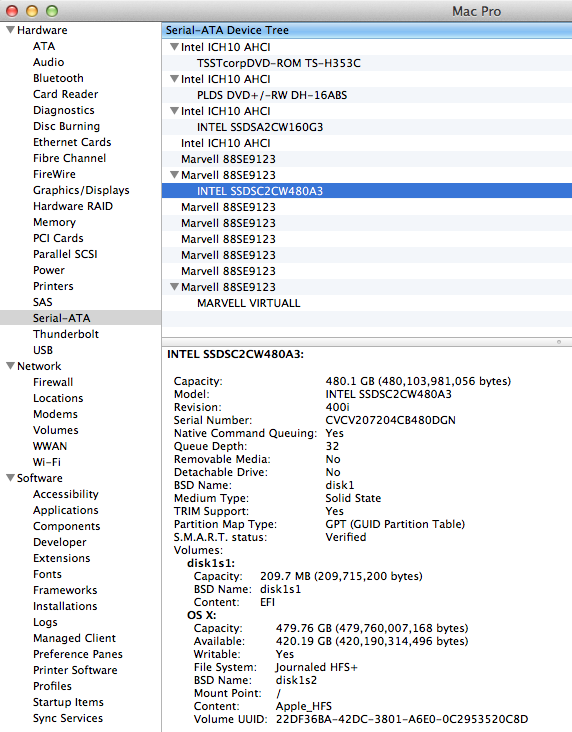
\includegraphics[scale=0.65]{trim.png}


\end{document}